\documentclass[conference]{IEEEtran}
\IEEEoverridecommandlockouts
\usepackage{cite}
\usepackage{amsmath,amssymb,amsfonts}
\usepackage{graphicx}
\usepackage{textcomp}
\usepackage{booktabs}
\usepackage{array}
\usepackage{url}
\def\BibTeX{{\rm B\kern-.05em{\sc i\kern-.025em b}\kern-.08em
    T\kern-.1667em\lower.7ex\hbox{E}\kern-.125emX}}

\begin{document}

\title{Learned Query Routing for Urdu News Search:\\
Two Indexes, Confidence Mixing, and a Negative Retrieval Result}

\author{\IEEEauthorblockN{1\textsuperscript{st} Hashim Shazad}
\IEEEauthorblockA{\textit{Dept.\ of Creative Technologies} \\
\textit{Air University}\\
Islamabad, Pakistan \\
abbasihashim30@gmail.com}
\and
\IEEEauthorblockN{2\textsuperscript{nd} Adnan Aslam}
\IEEEauthorblockA{\textit{Dept.\ of Creative Technologies} \\
\textit{Air University}\\
Islamabad, Pakistan}
}

\maketitle

\begin{abstract}
ULTRA routes Urdu news queries with a 150-character cutoff. That switch is easy to code and easy to fool: a short why-question can need the article, and a long fact-question can be answered by a headline. We keep the SHORT/LONG split but redefine it as retrieval need, score it with an eight-feature SVM, and open one of two indexes (headlines vs.\ full articles). Confidence mixes the rooms when the classifier is unsure. On a frozen 50-query set the SVM reaches 86\% against 84\% for a six-word rule (McNemar $p=1.0$). On 40 trap queries it reaches 60\% against 20\% for word count and 50\% for $\theta=150$ (McNemar 16--0), but almost all of that gain sits in 18 queries with why/how/fact wording. Dual-index P@5 on the same 40 queries does not follow the classifier (word count 36.50\%, SVM 33.00\%); nDCG@5 is highest if every query uses headlines. The cutoff is the wrong proxy. The SVM helps when the cue is visible. Early precision does not automatically follow.
\end{abstract}

\begin{IEEEkeywords}
Urdu information retrieval, query routing, support vector machine, dual-index search, Roman Urdu
\end{IEEEkeywords}

\section{Introduction}

Urdu search is not English search with a different font. Users mix Perso-Arabic script with Roman Urdu, spell the same word several ways, and pack an explanation request into three tokens~\cite{daud2017urdu,hussain2025qlora}. ULTRA~\cite{bashir2026ultra} is a dual-embedding news retriever for that setting. Its router is a tape measure: 150 characters or more takes one path, the rest take another.

A six-word cutoff is the other obvious tape. Both tapes fail on the queries that hurt. \emph{team haar ka tajzia} is short and needs the story. \emph{aaj pakistan ka score kya hai} can look long and still be a headline question.

English work already treats routing as a learned decision between sparse, dense, or hybrid retrieval~\cite{arabzadeh2021predicting} and as complexity-aware retrieval-augmented generation~\cite{jeong2024adaptiverag}. Urdu now has better test collections than a decade ago~\cite{iqbal2021cure,butt2024urdumsmarco}, but those collections do not tell a system which index to open.

This paper asks a smaller question than beating a large language model at routing. Can SHORT vs.\ LONG mean \emph{headline enough} vs.\ \emph{need the article}? Can a cheap SVM learn that on Urdu and Roman Urdu? Does wiring the decision into two indexes move P@5? The first two parts work when the wording cooperates. The third, on the frozen traps we care about, does not.

\section{Related Work}

Daud et al.~\cite{daud2017urdu} mapped the usual Urdu NLP obstacles: script, morphology, data. They predate dense retrieval. CURE~\cite{iqbal2021cure} and Urdu MS MARCO~\cite{butt2024urdumsmarco} give evaluation resources, not a router. Roman Urdu work is mostly classification~\cite{hussain2025qlora,mehmood2020xtreme}. Low-resource dense retrieval is known to sag once a language leaves the pretraining head~\cite{wu2024crosslingual,conneau2020xlmr}.

Adaptive routing is mature in English. Arabzadeh et al.~\cite{arabzadeh2021predicting} pick sparse vs.\ dense per query. Jeong et al.~\cite{jeong2024adaptiverag} escalate RAG by predicted complexity. ULTRA~\cite{bashir2026ultra} is the Urdu-specific starting point, and it still uses length. We keep ULTRA's corpus and encoder and change the switch.

\section{Method}

\subsection{What SHORT and LONG mean}

SHORT: a competent headline could answer the user (score, price, date, who won). LONG: they asked for why, how, impact, or a story. Labels are not token counts. If they were, a six-word rule would be unbeatable by construction.

\subsection{Two rooms and three lights}

Headlines and full articles are two dense indexes. Both use \texttt{paraphrase-multilingual-MiniLM-L12-v2}~\cite{reimers2019sbert}. The full-article room is Chroma collection \texttt{urdu\_news} over 111,860 news documents. The headline room is a separate title index. The same encoder is frozen; we did not swap it after seeing scores.

An RBF SVM~\cite{cortes1995svm} on eight z-scored features (Urdu ratio, Roman ratio, has-Urdu, has-Roman, token count, character count, mixed-script, Urdu character count) outputs a class and a Platt probability~$C(q)$~\cite{guo2017calibration}. HIGH ($C\geq 85\%$) searches only the chosen room. MEDIUM ($60$--$85\%$) mixes both. LOW ($<60\%$) expands the query and then mixes. LOW is implemented. On the small live probe used for defense it did not fire.

Roman Urdu is mapped with a word list. The file on disk has 198 pairs. Older drafts said 179. Native-script Urdu skips that step.

A later twelve-feature pickle exists in the demo. It is not the Phase~3B scorer. Mixing the two is how a 96\% figure appears. We do not report 96\%.

\begin{figure}[t]
\centering
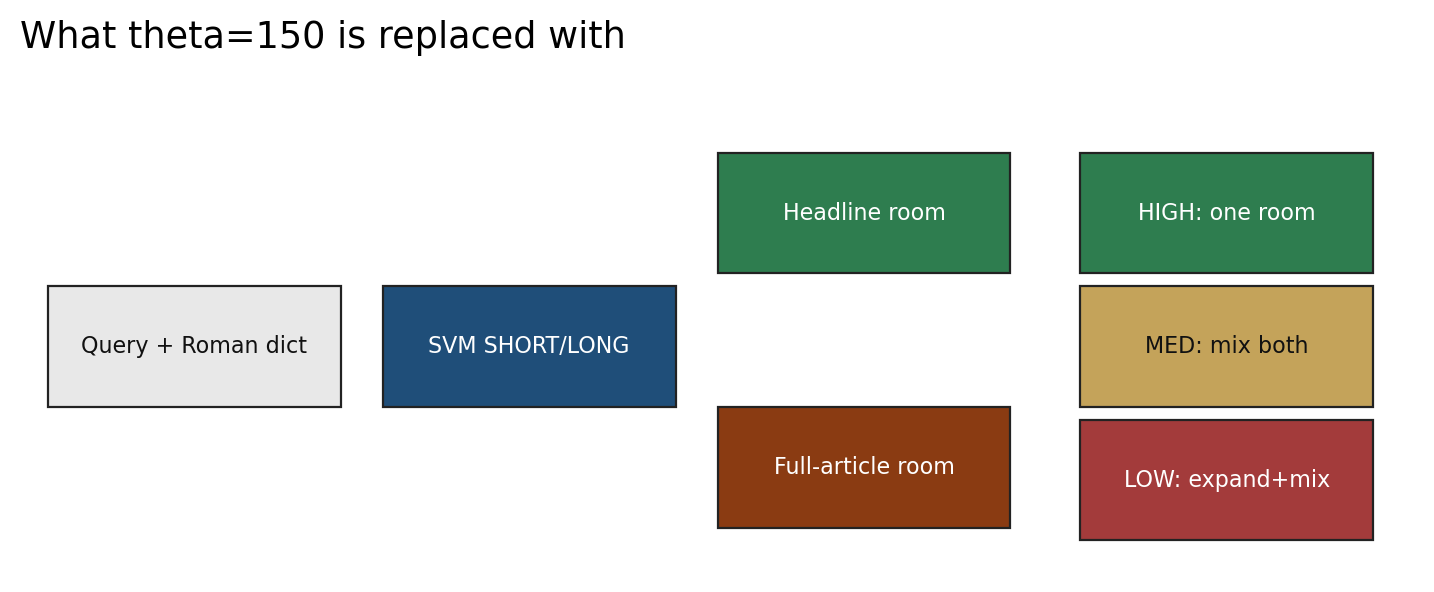
\includegraphics[width=\columnwidth]{figures/two_rooms_lights.png}
\caption{Router used in the frozen tests: dictionary, SVM room choice, HIGH/MEDIUM/LOW mixing.}
\label{fig:rooms}
\end{figure}

\section{Experiments}

Three layers are frozen and not averaged. Table~\ref{tab:cls} is the scorecard.

\textit{Development / CV.} Shows the task is learnable. Some splits hit 100\% vs.\ 50\% for $\theta=150$. Not the paper headline.

\textit{Phase 3B.} V2, eight features, 50 primary queries held out from a 409-query training pool. Word-count baseline ($\geq 6$ tokens $\rightarrow$ LONG) frozen before scoring.

\textit{Traps H001--H040.} Need labels, never used to train V2. Classification and dual-index P@5 (depth 5, 400 graded judgments: 0/1/2). Metrics: accuracy, exact McNemar, P@5, nDCG@5.

\section{Results}

\subsection{Classification}

Development 100\% is real and uninteresting. Frozen Phase~3B is 86\% vs.\ 84\% (McNemar 2 vs.\ 1, $p=1.0$). If that were the only table, we would stop.

On the traps the SVM reaches 60\%, word count 20\%, $\theta=150$ 50\% (McNemar 16--0, $p<0.001$). The cue split is the catch. Eighteen queries fire why/how/fact wording: SVM 18/18, word count 2/18. The other 22: both systems 27.27\% (Fig.~\ref{fig:cue}). The trap win is ``the SVM notices certain words,'' not ``the SVM understands need.''

\begin{table}[t]
\caption{Frozen classification. Do not mix with development 100\%.}
\label{tab:cls}
\centering
\begin{tabular}{lccc}
\toprule
\textbf{Layer} & \textbf{SVM} & \textbf{WC} & \textbf{$\theta{=}150$} \\
\midrule
Phase 3B ($n{=}50$) & 86\% & 84\% & -- \\
Traps ($n{=}40$) & 60\% & 20\% & 50\% \\
Traps, cue ($n{=}18$) & 100\% & 11.11\% & -- \\
Traps, no cue ($n{=}22$) & 27.27\% & 27.27\% & -- \\
\bottomrule
\end{tabular}
\end{table}

\begin{figure}[t]
\centering
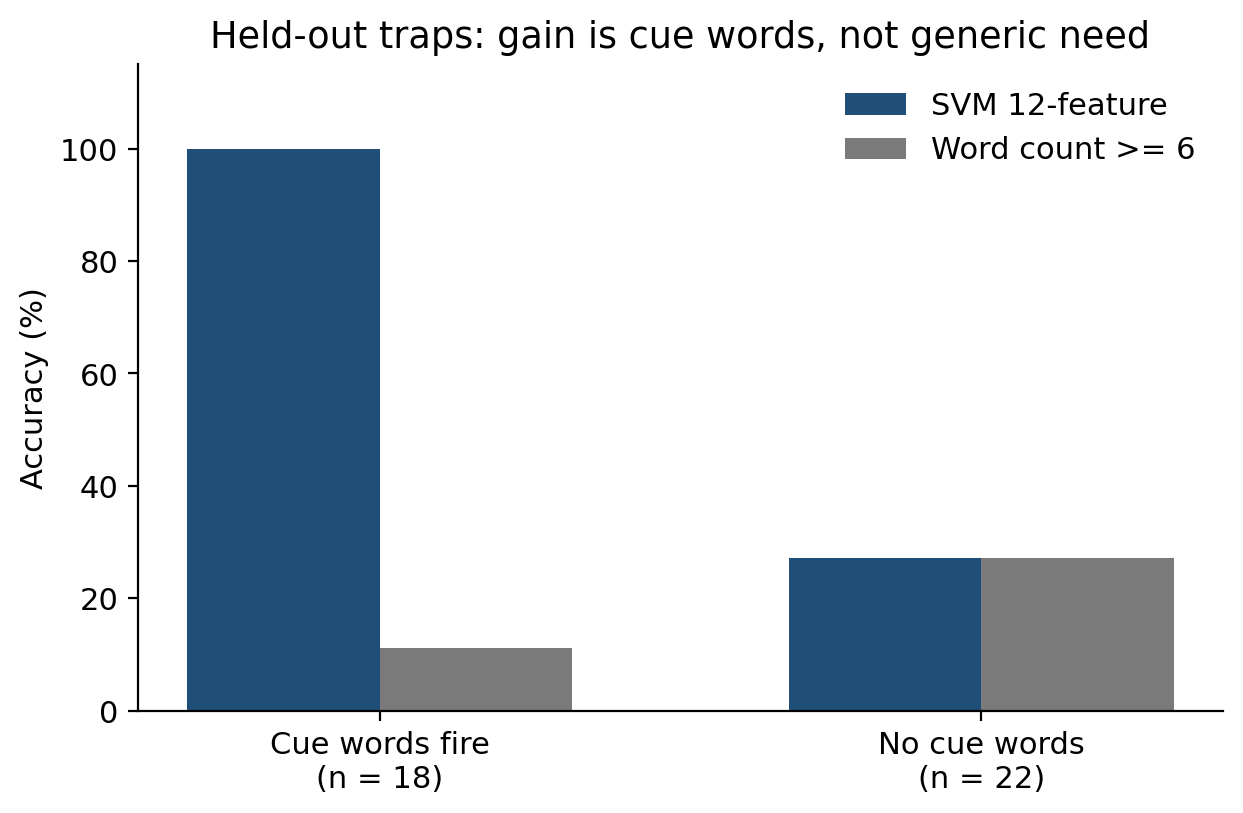
\includegraphics[width=\columnwidth]{figures/cue_split.png}
\caption{Trap cue split ($n=40$). Gain lives in why/how/fact wording.}
\label{fig:cue}
\end{figure}

\subsection{Retrieval}

Table~\ref{tab:p5} is the result that almost got edited out. Word count has the best P@5 (36.50\%). Always-headline and $\theta=150$ tie at 35.00\% (every query is SHORT under the character rule). Always-full is 34.25\%. The SVM is last at 33.00\%. nDCG@5 ranks always-headline first (0.6868). A smaller Phase~2.5 run ($n=33$) had a tiny SVM edge (35.76\% vs.\ 35.15\%). We do not stack it on the frozen 40.

\begin{table}[t]
\caption{Dual-index retrieval on H001--H040 (400 judgments, cutoff 5).}
\label{tab:p5}
\centering
\begin{tabular}{lcccc}
\toprule
\textbf{Router} & \textbf{P@5} & \textbf{nDCG@5} & \textbf{$\to$H} & \textbf{$\to$F} \\
\midrule
Word count $\geq 6$ & 36.50\% & 0.6476 & 20 & 20 \\
Always headline / $\theta{=}150$ & 35.00\% & 0.6868 & 40 & 0 \\
Always full article & 34.25\% & 0.6020 & 0 & 40 \\
SVM (V2) & 33.00\% & 0.6149 & 20 & 20 \\
\bottomrule
\end{tabular}
\end{table}

\begin{figure}[t]
\centering
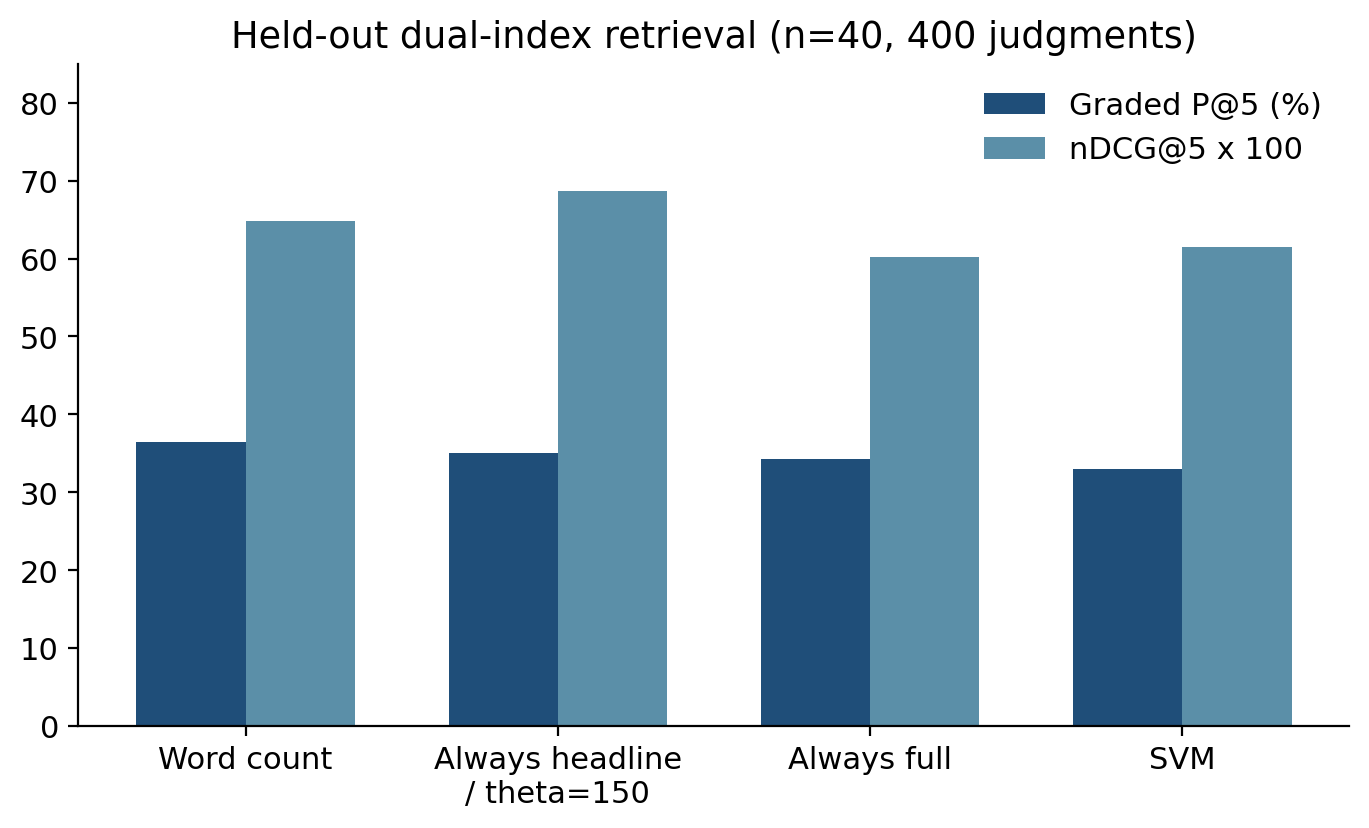
\includegraphics[width=\columnwidth]{figures/heldout_p5.png}
\caption{Held-out dual-index P@5. Classification win does not transfer.}
\label{fig:p5}
\end{figure}

\section{Discussion}

Reading A: character length is the wrong switch. A small SVM can beat word count on queries written to punish that rule, provided the cue split is printed next to the 16--0 table. We believe Reading A.

Reading B: therefore the first page of results gets better. We do not have Reading B. Need labels are not MiniLM rank labels. Headlines already carry the lexical overlap this encoder likes. Mixing rooms on medium confidence can import junk. Forty queries is a small IR test. All of that can be true at once.

Do not ship $\theta=150$ and call it adaptive. Do not ship this SVM and promise a better first page. If the product need is ``don't embarrass yourself on why/how queries,'' the cue features are doing real work. If the product need is nDCG, start with headlines and spend the next month on the encoder and the judgments.

Limitations are ordinary and binding: news only; a word list not a transliterator; no second independent rater; deployed 12-feature pickle $\neq$ frozen V2; LOW rarely fires; P@5 cannot see rank 8.

\section{Conclusion}

We replaced ULTRA's 150-character switch with a need-based SHORT/LONG label, an eight-feature SVM, two indexes, and a confidence mixer. The SVM is easy to beat word count with when the query contains why/how/fact wording, and it is not when those words are absent. Wiring the decision into retrieval did not improve P@5 on 40 frozen traps. nDCG@5 favored searching headlines for every query. That is the paper. It is enough to stop quoting character thresholds as a theory of the user. It is not enough to declare Urdu news search solved.

\section*{Acknowledgment}

This manuscript is the IEEE-format version of MS thesis work at Air University, Islamabad, under Dr.\ Adnan Aslam. It is prepared for submission to an IEEE conference or journal. It is not yet an IEEE Xplore publication.

\begin{thebibliography}{00}
\bibitem{daud2017urdu} A.\ Daud, W.\ Khan, and D.\ Che, ``Urdu language processing: a survey,'' \emph{Artif.\ Intell.\ Rev.}, vol.\ 47, pp.\ 279--311, 2017.
\bibitem{hussain2025qlora} N.\ Hussain \emph{et al.}, ``Fine-tuning large language models with QLoRA for offensive language detection in Roman Urdu-English code-mixed text,'' arXiv:2510.03683, 2025.
\bibitem{bashir2026ultra} A.\ Bashir, F.\ Qaiser, and I.\ Hussain, ``ULTRA: Urdu language transformer-based recommendation architecture,'' arXiv:2602.11836, 2026.
\bibitem{arabzadeh2021predicting} N.\ Arabzadeh, X.\ Yan, and C.\ L.\ A.\ Clarke, ``Predicting efficiency/effectiveness trade-offs for dense vs.\ sparse retrieval strategy selection,'' in \emph{Proc.\ CIKM}, 2021, pp.\ 2862--2866.
\bibitem{jeong2024adaptiverag} S.\ Jeong \emph{et al.}, ``Adaptive-RAG: learning to adapt retrieval-augmented large language models through question complexity,'' in \emph{Proc.\ NAACL}, 2024, pp.\ 7036--7050.
\bibitem{iqbal2021cure} M.\ Iqbal, B.\ Tahir, and M.\ A.\ Mehmood, ``CURE: collection for Urdu information retrieval evaluation and ranking,'' arXiv:2011.00565, 2021.
\bibitem{butt2024urdumsmarco} U.\ Butt, S.\ Varanasi, and G.\ Neumann, ``Enabling low-resource language retrieval: establishing baselines for Urdu MS MARCO,'' arXiv:2412.12997, 2024.
\bibitem{mehmood2020xtreme} F.\ Mehmood \emph{et al.}, ``A precisely Xtreme-multi channel hybrid approach for Roman Urdu sentiment analysis,'' arXiv:2003.05443, 2020.
\bibitem{wu2024crosslingual} J.\ Wu, Z.\ Ren, and S.\ Verberne, ``What are the limits of cross-lingual dense passage retrieval for low-resource languages?'' arXiv:2408.11942, 2024.
\bibitem{conneau2020xlmr} A.\ Conneau \emph{et al.}, ``Unsupervised cross-lingual representation learning at scale,'' in \emph{Proc.\ ACL}, 2020, pp.\ 8440--8451.
\bibitem{reimers2019sbert} N.\ Reimers and I.\ Gurevych, ``Sentence-BERT: sentence embeddings using Siamese BERT-networks,'' in \emph{Proc.\ EMNLP}, 2019, pp.\ 3982--3992.
\bibitem{cortes1995svm} C.\ Cortes and V.\ Vapnik, ``Support-vector networks,'' \emph{Machine Learning}, vol.\ 20, no.\ 3, pp.\ 273--297, 1995.
\bibitem{guo2017calibration} C.\ Guo, G.\ Pleiss, Y.\ Sun, and K.\ Q.\ Weinberger, ``On calibration of modern neural networks,'' in \emph{Proc.\ ICML}, 2017, pp.\ 1321--1330.
\end{thebibliography}

\end{document}
